\chapter{System Architecture and Development} \label{sec:systemdevelopment}

In the previous chapter I presented the requirements the solution had to achieve and evaluated different development options, discussing their advantages and disadvantages.
I closed the chapter with a solution proposition, where I justified hardware and software choices.
In this chapter I will present the implementation of such solution, going through the architecture design, configuration and development. 

\section{Architecture}

The architecture identically follows the EPCGlobal example, presented in figure~\ref{fig:archstructure} on chapter~\ref{sec:epcglobal}.
A detailed overview of the architecture is illustrated in figure~\ref{fig:practicalarchitecture}.

\begin{figure}
    \centering
    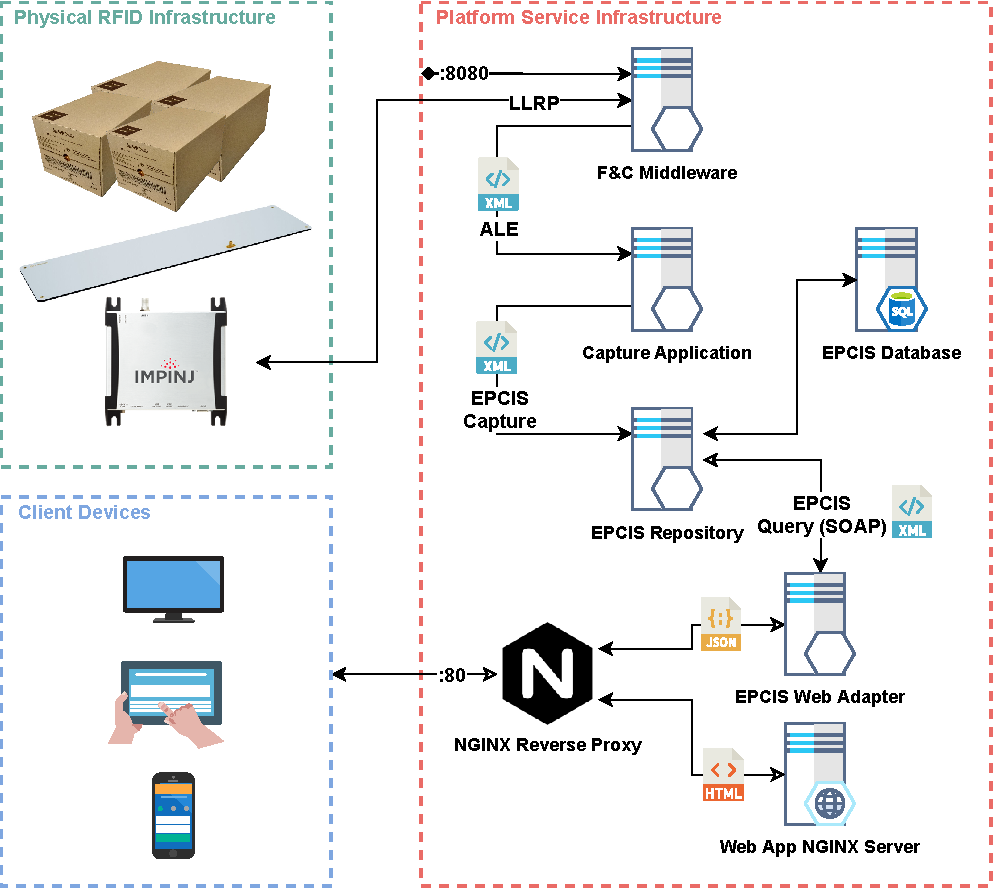
\includegraphics[width=\textwidth]{figs/platform_diagram.pdf}
    \caption{Overview of the solution architecture developed in this dissertation} 
    \label{fig:practicalarchitecture}
\end{figure}

The Impinj Speedway R120 reader and Keonn Advantenna-p14 are attached behind the bottom shelf, as shown in figure~\ref{fig:shelvephoto}, radiating the entire shelve.
The reader interrogates the tags, using the \ac{gen2} Tag Air Standard, following the active \acp{rospec} configured prior to the inventory.
The inventory information is sent inside \texttt{RO\_ACCESS\_REPORT} messages, to the \ac{llrp} interface of the middleware.

\begin{figure}
    \centering
    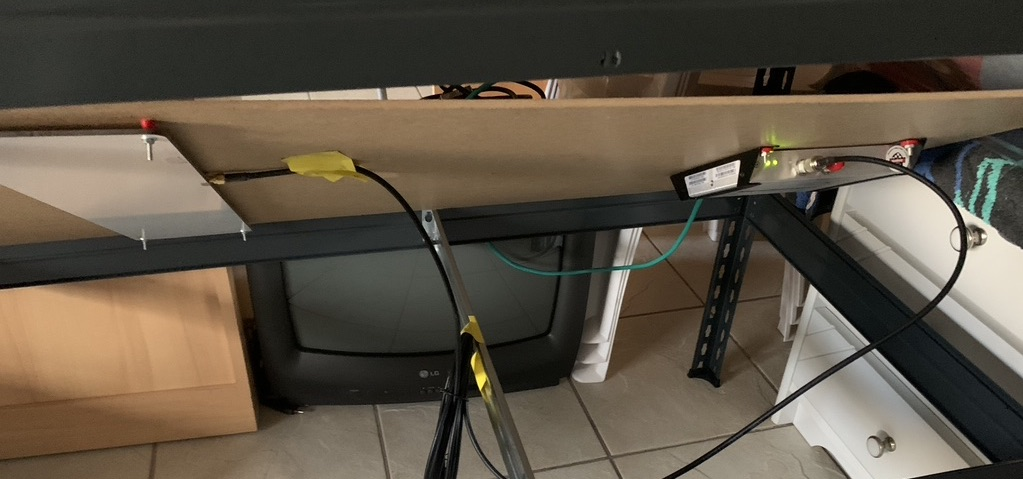
\includegraphics[width=\textwidth]{figs/completeshelve_photo.jpeg}
    \caption{Photograph of the Keonn Advantenna-p14 and Impinj Speedway R120 attached behind the bottom shelf}
    \label{fig:shelvephoto}
\end{figure}

The Fosstrak \ac{fc} middlware receives the inventory information from the reader, processes it, following the configured \acp{ecspec}, and periodically generates \acp{ecreport}, which are sent to the capture application \ac{ale} capture interface.

The Fosstrak capture application receives the \acp{ecreport}, contextualizes them and runs additional business logic. The contextualized data is aggregated in \acs{epcis} event documents, following the \ac{cbv} vocabulary guidelines, and sent to the \ac{epcis} repository.

The \ac{epcis} repository permanently saves the \ac{epcis} data in to the \ac{epcis} database. The \ac{epcis} repository exposes the \ac{soap} query interface, which can be used to retrieve information.

The managing application to visualize the smart shelve inventory, was made using web technologies. The application is served to browsers by an NGINX static file server. The browser running the application queries the data in the \ac{epcis} repository.
Modern browsers do not support \ac{soap} natively. 
To mitigate this problem, the requests pass through a crude \ac{epcis} web adapter, serving as a proxy between web applications and the \ac{epcis} repository. 
The proxy adapts the \ac{soap} \ac{xml} requests into \ac{http} and \ac{json} endpoints, which modern browsers understand.

All client requests hitting the platform go through an NGINX reverse proxy. This hides the topology and characteristics of the back-end servers, removing the direct internet access to them. The services on the platform are kept inside a non-public subnet and concentrate the access control on that single point. The NGINX server also allows load balancing between the services, which is useful when there is a need to scale the platform. The proxy also deals with cross-origin resource sharing mechanism, freeing the servers from dealing with it.

All services in the platform infrastructure are containerized using Docker, and orchestrated using Docker Compose. The yaml compose file, containing the description of  can be consulted in appendix~\ref{apx:composefile}.

\section{\acs{epc} Serialization Plan}

When companies adhere to the EPCGlobal framework, there are a few things that have to be deliberated.
One of those is delineating the \acs{epc} serialization plan, where an evaluation of unique products and serial numbers is made.
The plan has to ensure that a company has enough unique product numbers to identify current and future products.

In the case of this dissertation, the serialization plan was already performed by Nespresso.
Each of their products has already an assigned \ac{gtin}, including the cardboard case for transport.

From the product cases for transport are identified by the GS1-$128$ barcode, and sleeves by \acs{ean}-$13$ barcode. From those used for testing, two Nespresso company prefixes were present: $76300544$ and $76300396$ respectively. Nestlé Nespresso SA has many more registered. Searching in GS1 Company Database (GEPIR), I found $18$ more, registered in Switzerland.
From the \acs{ean}-$13$ barcode in sleeves, the \acs{gtin}-$13$ can be inferred and converted to \acs{gtin}-$14$ for \ac{sgtin}-$96$ encoding on \ac{gen2} \ac{epc} \acs{rfid} tags, which was covered in section~\ref{sec:sgtin}.
For the GS1-$128$ barcode in product cases for transport, an example of the barcode deconstruction is illustrated in figure~\ref{fig:gs1-128barcode}.

\begin{figure}
    \centering
    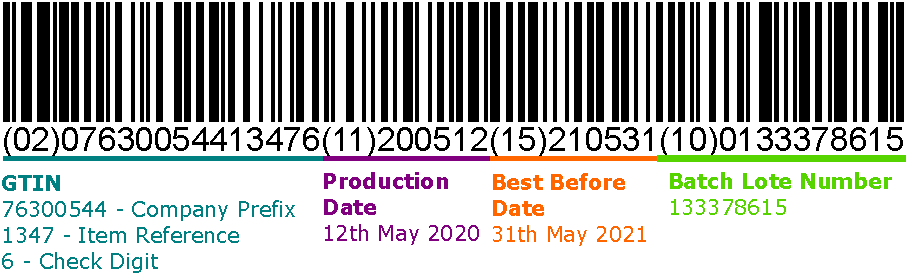
\includegraphics[width=\textwidth]{figs/gs1-128barcode.pdf}
    \caption{Deconstruction of a GS1-$128$ barcode from a Volluto coffee cardboard case for transport used in this dissertation has a test product (GS1 AI IDs on \acs{tds} Section F.1~\cite{EPCTagData})}
    \label{fig:gs1-128barcode}
\end{figure}

With the \acs{gtin}-$14$, it is possible to encode \ac{sgtin}-$96$ in \ac{gen2} tags. To write the \acp{epc} in the testing tags, it was used the Impinj Octane Java SKD \texttt{WriteEpc.java} sample code, adapted with the \ac{tdt} engine. Instead of generating a random \ac{epc}, the Fosstrak \ac{tdt} engine was used to encode a valid \ac{epc} with the correspondent company prefix, item reference and serial in to hexadecimal, which can be passed to the \texttt{TagWriteOp} class to configure the reader and program the tag.

A tag was attached to each sleeve and transport box, with their correspondent \ac{gtin} and unique serial number as a \ac{sgtin}-$96$.

\section{Reader}

Throughout this dissertation, the reader was configured employing three approaches: using the Impinj Octane Java SDK~\cite{OctaneSDK}, the Impinj LTK using \ac{xml} configuration files~\cite{LTKXMLJava} and with Fosstrak \ac{llrp}Comander client software~\cite{FosstrakLLRPCommander}.
Each one has their advantages and disadvantages.

In section~\ref{sec:llrp}, I mentioned that \ac{xml} is used to provide a human readable and abstract the \ac{llrp} standard.
In fact, it can be used to describe messages like the \textit{ADD\_ROSPEC} and \textit{SET\_READER\_CONFIG}.
This makes it easy to create and manage configuration files compared to code, which requires knowledge of each reader manufactured SDK and referent programming language, to to maintain.

When configuring the reader with the \acs{llrp}Commander or LTK-\ac{xml}, the configurations can be interchangeable, sharing the same \ac{xml} file. These methods have a few flaws. From what I experienced, \ac{llrp}Commander has some problems dealing with Impinj extensions and filter parameters, and requires Eclipse $3.3$ 2007 build, which is old and not maintained.
The Impinj LTK-\ac{xml} configuration method also seems to have some problems dealing with Impinj extensions~\footnote{Example: specifying \texttt{ImpinjInventorySearchMode} returns unable to convert LTK-XML to Internal Object. \texttt{C1G2InventoryCommand} has unknown element \texttt{ImpinjInventorySearchMode} which exists and is documented~\cite{ImpinjLTKProgrammers}}.

The suggested approach is using the Octane SKD. It forfeits the advantages of a \ac{xml} configuration file, but it provides all the features expected from the reader, and is reliable and fast to configure.
Octane 6.2.0, last version at the time of this dissertation, is based on \ac{llrp} version 1.0.1, which does not support some Class 1 \ac{gen2} version 1.2.0 features natively in the \ac{llrp} LTK implementation~\cite{ImpinjOctaneLLRP}. Octane includes vendor extensions in the SDK to expose the underlying air protocol features.
The reader firmware used was version 5.12.2.240 (Build cbc9ad1d0d1).

The full code used to configure the reader can be consulted in appendix~\ref{apx:octanereaderconfig}.
The \ac{xml} configuration files used with \ac{llrp}Commander and LTK-\acs{xml} program can be consulted in appendix~\ref{apx:xmlreaderconfig}.
The parameters configuration will be discussed in the next section.

\subsection{Configuration}

In section~\ref{sec:llrpspecs} I presented the \ac{rospec} used to control the reader operation through the \ac{llrp} protocol. The \ac{rospec} defined for this solution will be discussed in detail in this section.
Use appendix~\ref{apx:xmlreaderconfig} \ac{xml} configuration files as reference.

\subsubsection{Antenna configuration}

It is good practice in \ac{uhf} \ac{rfid} systems to configure antennas aside from the \ac{rospec} definition. \ac{rf} antenna parameters are dependent on \ac{rfid} hardware and environment in which the system is deployed. \acp{rospec} allow antenna configuration, but should only specify reader control operation, namely inventory logic operations. This ensures configuration interoperability between same logic deployments in disparate \ac{rf} environments.

To do so, \ac{llrp} defines the \textit{SET\_READER\_CONFIG} message with the \texttt{AntennaConfiguration} parameter.
This parameter contains a few important parameters and fields:

\texttt{ReceiverSensitivity} specifies the effective receive sensitivity level in dBm. While testing the solution, the \ac{rf} environment conditions were optimal, which allowed setting the reader to the maximum sensitivity of $-80$dBm. This sensitivity is index $1$ on the \texttt{ReceiveSensitivityTableEntry}. For the R120 reader capabilities consult appendix~\ref{apx:readercapabilities}.
\texttt{TransmitPower} specifies the transmission power provided to the antennas as an offset into the \texttt{TransmitPowerLevelTableEntry}. For the Speedway R120 reader power with PoE, the maximum transmission power is $30$ dBm, which is index of $81$, used in this dissertation tests~\cite{ImpinjOctaneLLRP, SettingReceiveSensitivity}.

The \texttt{C1G2InventoryCommand} parameter is were the Class 1 \ac{gen2} air protocol is tunned.
\texttt{TagInventoryStateAware} flag is used to determine how to process all the \texttt{C1G2Filter} and \texttt{C1G2Singulation} parameters in this command~\footnote{At a functional level, if the Client is managing the tag states during an inventory operation (i.e\ the Client is specifying Class1 \ac{gen2} tag Select command Target and Action values), then it will set that flag to true and pass the appropriate fields in the C1G2 Filter and C1G2 Singulation parameters. If a reader set \texttt{CanDoTagInventoryStateAwareSingulation} to False in LLRPCapabilities, then the Reader shall ignore the \texttt{TagInventoryStateAware} flag~\cite{LowLevelReader}}.

The \texttt{C1G2RFControl} parameter specifies Speedway Gen2 modes selected by Impinj system engineering to provide the best performance. No Tari adjustment is necessary. Tari values passed by the client will be ignored~\cite{ImpinjOctaneLLRP}.

\texttt{ModeIndex} selects the operation mode~\cite{ReaderModesMade, ImpinjOctaneLLRP}. For the use case of this dissertation, it can be one of the three bellow, depending on the \ac{rf} environment in which the system is deployed: 

\begin{itemize}
    \item $1002$ (AutoSet Dense Reader Deep Scan) configures the Reader to choose the best \ac{gen2} link parameters for the environments where the tag population is relatively static and we wish to attempt to search for the weakest tag~\cite{ReaderMode1002};
    \item $1003$ (Autoset Static Fast) is an adaptation of Autoset Dense Reader Deep Scan for good \ac{rf} environments;
    \item $1004$ (AutoSet Static Dense Reader) is an adaptation of Autoset Dense Reader Deep Scan for difficult \ac{rf} environments.
\end{itemize}

The option used was \texttt{ModeIndex} $1002$. The $1004$ is not currently available for the R120 in the ETSI european \ac{uhf} band. The $1003$ does not provide confidence in warehouse malls, where other readers systems can operate and create poor \ac{rf} environment conditions.

Impinj offers a few custom parameters supported in Octane \ac{llrp}, namely the \texttt{ImpinjInventorySearchMode}, a Impinj-specific inventory search mode. 
To understand search modes, we have to understand sessions. This thematic goes deep in to the \ac{gen2} air protocol and will only briefly contextualized. \ac{gen2} defines up to four tag sessions. Sessions are states tags can transit to, in order to help the reader attempt to singulate, i.g\ read, tags.
Sessions can be used to determine when a tag will respond to a query from the reader, and/or allow tags to maintain independent states when communicating with multiple readers at the same time. 

Impinj readers implement state unaware singulation, in that they provide a high-level control over the search algorithm, through \texttt{ImpinjInventorySearchMode} parameter, not interfering with any of the standard \ac{llrp}/\ac{gen2} settings~\cite{ImpinjOctaneLLRP, UnderstandingEPCGen2}.
Impinj search modes can be consulted in appendix~\ref{apx:searchmodes}.
In this dissertation we used Tag Focus to make sure every tag was read. This was possible only because we used HID 6H2E43 tags with use Monza chips in this dissertation. For generic tags I recommend using Single Target Inventory search mode.

Using purely \ac{llrp} settings for configuration interchangeability with other reader manufacturers, \ac{gen2} provides the \texttt{C1G2SingulationControl} to control the singulation process in the Class 1 \ac{gen2} air protocol:

\begin{itemize}
    \item Tag transit time: This is the measure of expected tag mobility in the field of view of the antenna where this inventory operation is getting executed.
    \item Tag population: This is the expected tag population in the field of view of the antenna.
    \item Session ID: This is the C1G2 session number that the tags use to update the inventory state upon successful singulation.
    \item  TagInventoryStateAwareSingulationAction: This is not used since the TagInventoryStateAware flag is set to false in the InventoryParameterSpec.
\end{itemize}

Configurations with tunning of these setting were done for testing, but were not used in the final prototype presented in this dissertation, so no further detail will be done.


\subsubsection{Operation configuration}

The \texttt{ROBoundarySpec} parameter carries the lifetime of the Reader inventory and survey operation.
ROSpecStartTrigger, ROSpecStopTrigger: This is the start and stop trigger for this ROSpec.

Used ROSpecStopTriggerType Periodic.
Periodic trigger values: period - Time period specified in milliseconds; offset - Time offset specified in milliseconds from receiving message to start. useful for one-shot inventory.

Used ROSpecStartTriggerType Periodic.

\textbf{Antenna inventory operations configuration (\ac{aispec})}

AISpecStopTrigger parameter defines the stop (i.e., terminating boundary) of an antenna inventory operation~\cite[sec. 11.2.2.1]{LowLevelReader}. Here it was set to Null to Stop when \ac{rospec} is done.

InventoryParameterSpec Configuration (C1G2InventoryCommand) \dots



\paragraph{Report Operation Report Spec (ROReportSpec)}

Describes the messages and parameters used in reports, event notifications and keepalives that are generated by the Reader and sent to the Client.

A reporting trigger (ROReportTrigger or AccessReportTrigger) generates a report while a connection is open.

In the use case in this dissertation we are not concerned with near real-time updates on the state of the inventory. So we can reduce the report generation by letting the end of the ROSpec generate a report periodically.
So ROReportTrigger can be set to \texttt{Upon\_N\_Tags\_Or\_End\_Of\_ROSpec} with N=0 (unlimited tag in antenna's field of view)~\cite[sec. 14.2.1]{LowLevelReader}

In terms of the content useful to retrieve from the reader inventory singulation, the ROSpecID, FirstSeenTimestamp, LastSeenTimestamp are in the interests of the application.

We can enable it the TagReportContentSelector block by setting the Enable in each on.

\paragraph{Tools}

Used Fosstrak \ac{llrp} Commander with the old old Eclipse 3.3 and JRE/JDK 1.8 to configure de reader using an xml schema.
Also developed a java tool to configure the reader using \ac{llrp}. Used the java llrp. LTK and code by impinj to configure it based on the "same" schema used in the LLRP commander.
In the java tool, the xml parser sometimes requires fields that shouldn't be needed because Impinj reader ignores then in certain configuration options. But for the configuration to be validated, they have to be present in order to validate de xsd schema (TagInventoryStateAware, Tari)

\section{Middleware}

\paragraph{LRSpec}

\paragraph{ECSpec}

We have 2 ec reports: one for informing the tag uri added and deleted from the shelve that will be used for the capture application to provide supply chain visualization to the epcis repository; a second for informing the real-time inventory service on the point of sale the current state of inventory (will sent counts for products).

ECSpec2: want only to know the number of which coffee type are available in storage, so SGTIN filter value of 1 (Point of Sale (POS) Trade Item), with nespresso's company prefix, different item references groups and any serial tag number in those groups.

%Table 10-1 in sec 10.2 TDS : Filter Values for SGTIN EPC Tags
%Ref ECReportOutputSpec in 8.2.10 ALE standard core

\section{Capture application}

\section{EPCIS repository}

\section{Managements application}